\section{Detailed RL and distillation objectives}
\label{app:objectives}

The notation and losses below expand the routed objective in Section~\ref{sec:method}.

For each hard prompt $x$, let $\{y_j\}_{j=1}^{G}$ denote its rollout group and
let $r_j=r(x,y_j)$ be the reward of response $y_j$. We compute the
group-relative advantage as
\begin{equation}
  A_i
  =
  \frac{r_i-\overline r_x}{\sigma_x+\epsilon_{\mathrm{adv}}},
  \qquad
  \overline r_x
  =
  \frac{1}{G}\sum_{j=1}^{G}r_j,
  \qquad
  \sigma_x
  =
  \sqrt{
    \frac{1}{G}
    \sum_{j=1}^{G}
    (r_j-\overline r_x)^2
  }.
  \label{eq:group-relative-advantage}
\end{equation}
For a response $y_i$ of length $T_i$, let
$s_{i,t}=(x,y_{i,<t})$ denote its prefix at token $t$. The importance ratio is
\begin{equation}
  \rho_{i,t}(\theta)
  =
  \frac{\pi_\theta(y_{i,t}\mid s_{i,t})}
       {\pi_{\mathrm{old}}(y_{i,t}\mid s_{i,t})}.
\end{equation}
Its sequence-level RL loss is
\begin{equation}
  \ell_i^{\mathrm{RL}}
  =
  -\frac{1}{T_i}
  \sum_{t=1}^{T_i}
  \min\left(
    \rho_{i,t}(\theta)A_i,\,
    \operatorname{clip}
    \bigl(\rho_{i,t}(\theta),1-\epsilon,1+\epsilon\bigr)A_i
  \right).
  \label{eq:rl-sequence-loss}
\end{equation}

For an easy response $y_i$, we consider three OPD variants. Two directly
optimize a top-$K$ KL objective, while the third estimates reverse KL through
policy gradients.

\paragraph{Supervised-gradient forward KL (SG-FKL).}
Let $\mathcal V_{i,t}^{K}$ denote the teacher's top-$K$ tokens at prefix
$s_{i,t}$. To ensure that termination behavior is supervised even when a stop token does not appear in the teacher's top-$K$ predictions, we augment this set with the stop-token set
$\mathcal V_{\mathrm{stop}}$:
\begin{equation}
  \widetilde{\mathcal V}_{i,t}^{K}
  =
  \mathcal V_{i,t}^{K}
  \cup
  \mathcal V_{\mathrm{stop}}.
\end{equation}

We normalize the teacher distribution over the augmented support:
\begin{equation}
  \bar\pi_k^{K}(v\mid s_{i,t})
  =
  \frac{
    \bar\pi_k(v\mid s_{i,t})
  }{
    \sum_{u\in\widetilde{\mathcal V}_{i,t}^{K}}
    \bar\pi_k(u\mid s_{i,t})
  },
  \qquad
  v\in\widetilde{\mathcal V}_{i,t}^{K}.
\end{equation}
Then, the forward-KL OPD objective is
\begin{equation}
  \ell_i^{\mathrm{SG\text{-}FKL}}
  =
  \frac{1}{T_i}
  \sum_{t=1}^{T_i}
  \sum_{v\in\widetilde{\mathcal V}_{i,t}^{K}}
  \bar\pi_k^{K}(v\mid s_{i,t})
  \left[
    \log\bar\pi_k^{K}(v\mid s_{i,t})
    -
    \log\pi_\theta(v\mid s_{i,t})
  \right].
  \label{eq:opd-sg-fkl}
\end{equation}
Gradients are taken directly through the student logits, while the teacher
distribution is detached.

\paragraph{Supervised-gradient reverse KL (SG-RKL).}
For the reverse direction, we also normalize the student distribution over
the same augmented support:
\begin{equation}
  \pi_\theta^{K}(v\mid s_{i,t})
  =
  \frac{
    \pi_\theta(v\mid s_{i,t})
  }{
    \sum_{u\in\widetilde{\mathcal V}_{i,t}^{K}}
    \pi_\theta(u\mid s_{i,t})
  },
  \qquad
  v\in\widetilde{\mathcal V}_{i,t}^{K}.
\end{equation}
We then directly minimize
\begin{equation}
  \ell_i^{\mathrm{SG\text{-}RKL}}
  =
  \frac{1}{T_i}
  \sum_{t=1}^{T_i}
  \sum_{v\in\widetilde{\mathcal V}_{i,t}^{K}}
  \pi_\theta^{K}(v\mid s_{i,t})
  \left[
    \log\pi_\theta^{K}(v\mid s_{i,t})
    -
    \log\bar\pi_k^{K}(v\mid s_{i,t})
  \right].
  \label{eq:opd-sg-rkl}
\end{equation}


\paragraph{Policy-gradient reverse KL (PG-RKL).}
The third objective only uses the teacher probability of the sampled token.
For each token, we define the detached OPD advantage
\begin{equation}
  A_{i,t}^{\mathrm{OPD}}
  =
  \operatorname{sg}\left[
    \log\bar\pi_k(y_{i,t}\mid s_{i,t})
    -
    \log\pi_{\mathrm{old}}(y_{i,t}\mid s_{i,t})
  \right],
  \label{eq:opd-advantage}
\end{equation}
where $\operatorname{sg}[\cdot]$ denotes stop-gradient. We then apply the
PPO-style clipped objective:
\begin{equation}
  \ell_i^{\mathrm{PG\text{-}RKL}}
  =
  -\frac{1}{T_i}
  \sum_{t=1}^{T_i}
  \min\left(
    \rho_{i,t}(\theta)A_{i,t}^{\mathrm{OPD}},
    \operatorname{clip}
    \bigl(\rho_{i,t}(\theta),1-\epsilon,1+\epsilon\bigr)
    A_{i,t}^{\mathrm{OPD}}
  \right).
  \label{eq:opd-pg-rkl}
\end{equation}

Let $\ell_i^{\mathrm{OPD}}$ denote the OPD loss used by a particular LSD
variant. Under sequence-mean--token-mean aggregation, we first average the
token losses within each response. We then average the resulting
sequence-level losses within their assigned routes:
\begin{equation}
  \overline{\ell}^{\mathrm{RL}}
  =
  \frac{1}{n_{\mathcal H}}
  \sum_{i\in\mathcal Y_{\mathcal H}}
  \ell_i^{\mathrm{RL}},
  \qquad
  \overline{\ell}^{\mathrm{OPD}}
  =
  \frac{1}{n_{\mathcal E}}
  \sum_{i\in\mathcal Y_{\mathcal E}}
  \ell_i^{\mathrm{OPD}},
  \label{eq:route-losses}
\end{equation}
where $\mathcal Y_{\mathcal H}$ and $\mathcal Y_{\mathcal E}$ contain the
response sequences routed to RLVR and OPD, respectively, and
$n_{\mathcal H}=|\mathcal Y_{\mathcal H}|$ and
$n_{\mathcal E}=|\mathcal Y_{\mathcal E}|$.

\clearpage
\subsection{Logged optimization diagnostics}
\label{app:training-diagnostics}

We examine the logged training histories of the three single-turn LSD
runs. The shared training
interval is steps 501--1628: SG-RKL's available training history begins
at step 501, and PG-RKL's ends at step 1628. All three configurations
record an EMA half-life of four updates, an EMA update interval of one,
and an online routing threshold of one.

\begin{figure}[htbp]
  \centering
  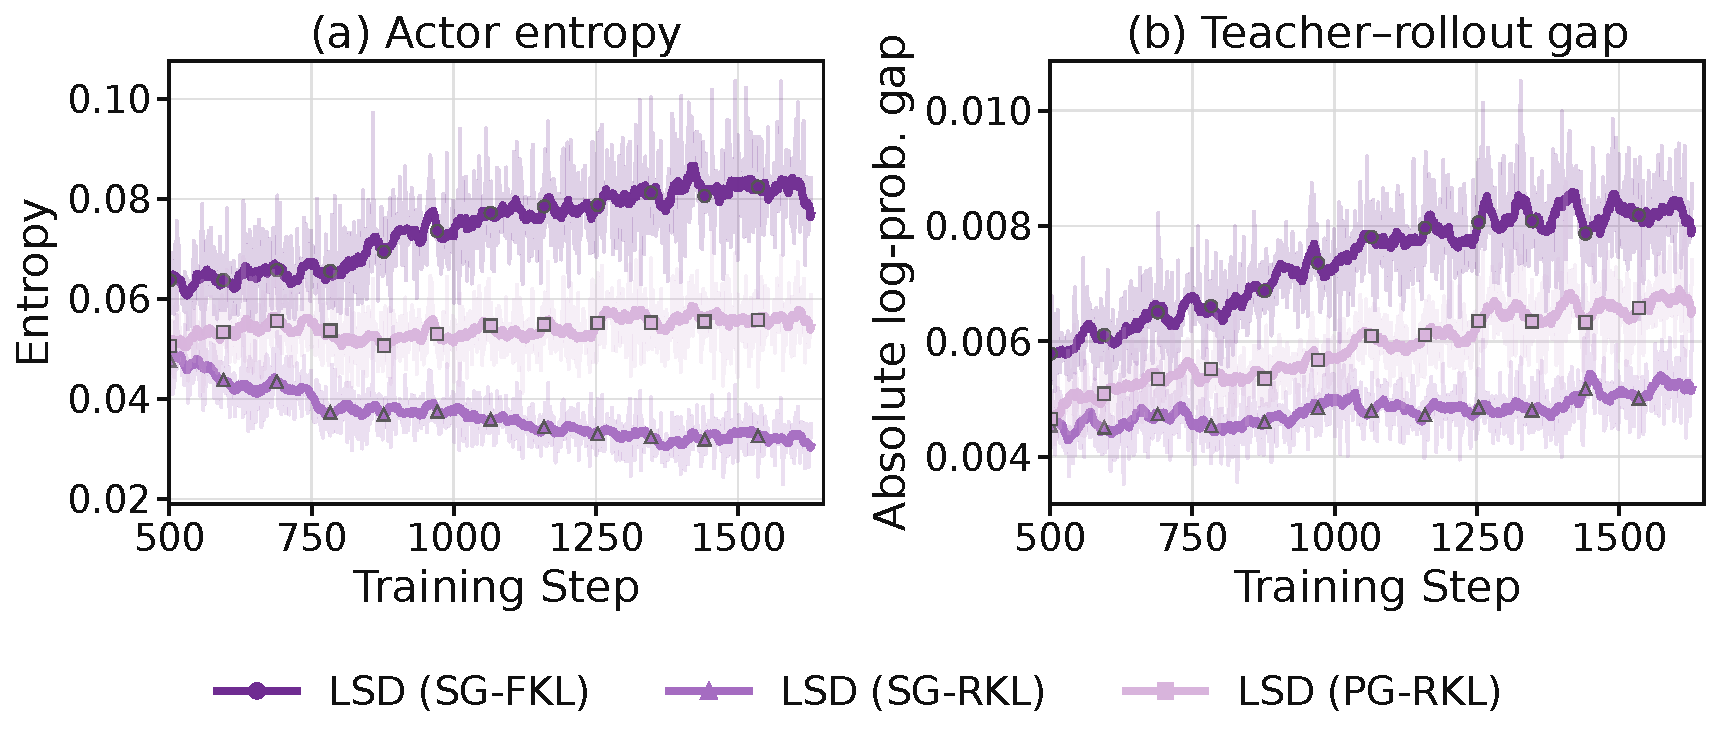
\includegraphics[width=\linewidth]{figures/wandb_objective_diagnostics.pdf}
  \caption{\textbf{Training dynamics of the three LSD objectives.}
  Actor entropy (left) and the mean absolute teacher--rollout
  log-probability difference before updates (right) over the shared
  steps 501--1628. Faint traces show raw per-step values; marked curves
  show centered 21-step means, using available points at the boundaries. SG-RKL exhibits
  lower entropy and a smaller teacher--rollout discrepancy over this
  interval. Each trajectory uses its own run's training batches.}
  \label{fig:objective-training-dynamics}
\end{figure}

\begin{table}[htbp]
  \centering
  \caption{\textbf{Optimization diagnostics over a shared training interval.}
  Values are arithmetic means of the logged per-step scalars over all
  1128 shared steps, without smoothing. These training steps are not
  independent experimental replicates.}
  \label{tab:objective-training-diagnostics}
  \small
  \begin{tabular}{lrrr}
    \toprule
    Variant & Actor entropy & Teacher--rollout gap & Easy sequences (\%) \\
    \midrule
    \methodname{SGFKL}{SG-FKL} & 0.0743 & 0.00738 & 21.51 \\
    \methodname{SGRKL}{SG-RKL} & 0.0367 & 0.00481 & 20.23 \\
    \methodname{PGRKL}{PG-RKL} & 0.0542 & 0.00590 & 20.67 \\
    \bottomrule
  \end{tabular}
\end{table}

\clearpage
\subsection{Easy and hard token allocation during training}
\label{app:training-token-routes}

The training histories directly record the fraction of sequences and
tokens assigned to each route. Figure~\ref{fig:training-token-routes}
shows their evolution and distribution over the 1128 shared steps
501--1628. The two route fractions sum to one at every recorded step,
up to numerical precision.

\begin{figure}[htbp]
  \centering
  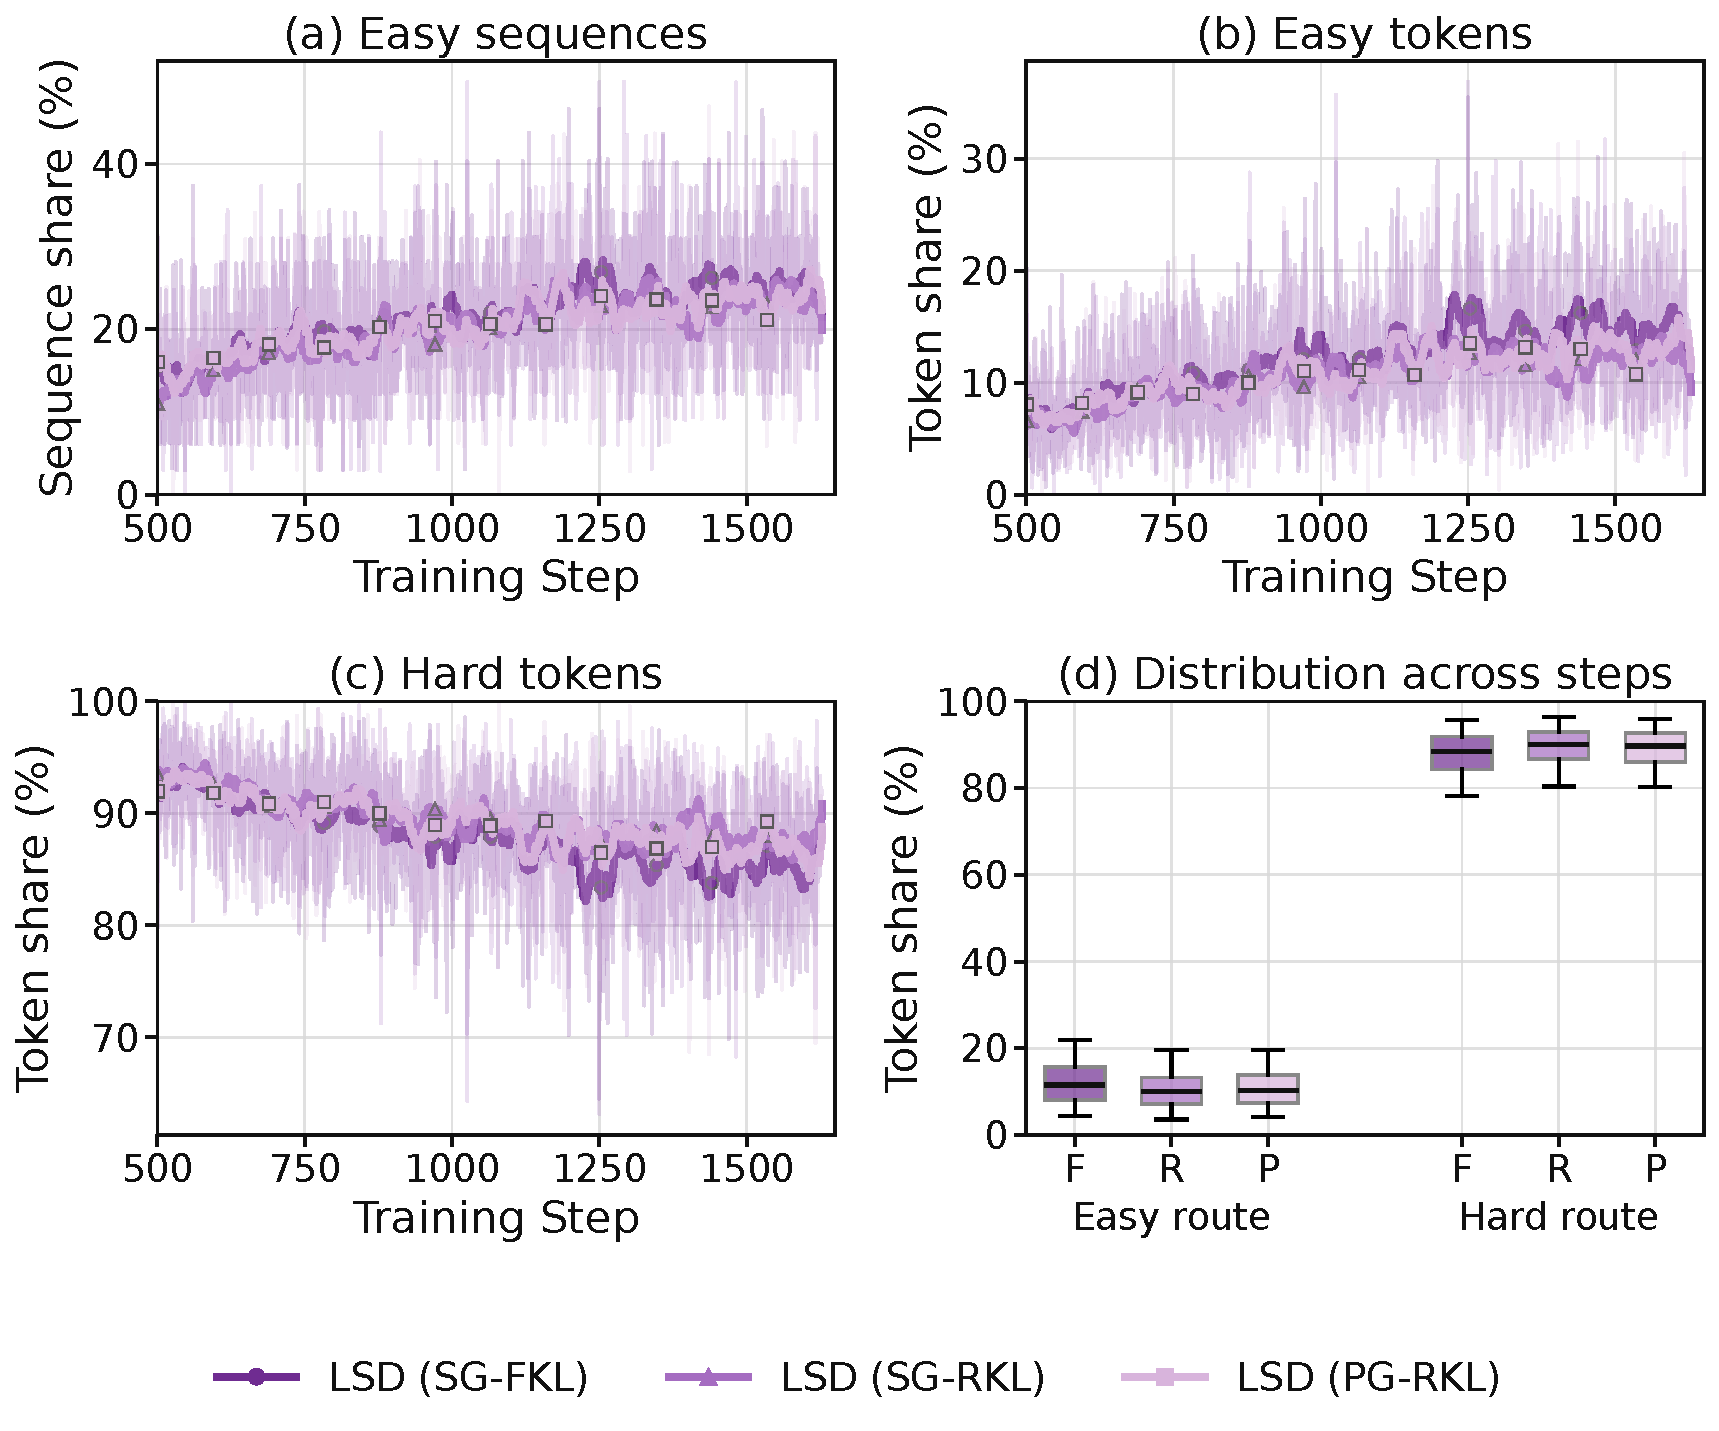
\includegraphics[width=\linewidth]{figures/wandb_training_token_routes.pdf}
  \caption{\textbf{Training token allocation between the easy and hard routes.}
  Panels (a)--(c) show raw per-step fractions and centered 21-step means.
  Panel (d) summarizes the distribution of token shares across training
  steps: boxes show the interquartile range and median, and whiskers
  show the 5th and 95th percentiles. F, R, and P denote SG-FKL, SG-RKL,
  and PG-RKL. These are distributions of per-step shares, not
  individual response lengths or uncertainty intervals.}
  \label{fig:training-token-routes}
\end{figure}

\begin{table}[htbp]
  \centering
  \caption{\textbf{Training-route allocation over steps 501--1628.}
  The first three numeric columns are means of logged per-step
  fractions, expressed in percent. The last reports the median and
  interquartile range of the easy-token share.}
  \label{tab:training-token-routes}
  \small
  \resizebox{\linewidth}{!}{%
  \begin{tabular}{lrrrr}
    \toprule
    Variant & Easy seq.\ (\%) & Easy tok.\ (\%) & Hard tok.\ (\%)
      & Easy tok.\ median [IQR] \\
    \midrule
    \methodname{SGFKL}{SG-FKL} & 21.51 & 12.17 & 87.83 & 11.54 [8.09, 15.67] \\
    \methodname{SGRKL}{SG-RKL} & 20.23 & 10.58 & 89.42 &  9.99 [7.11, 13.27] \\
    \methodname{PGRKL}{PG-RKL} & 20.67 & 10.94 & 89.06 & 10.29 [7.31, 13.90] \\
    \bottomrule
  \end{tabular}%
  }
\end{table}

The easy route accounts for a smaller share of tokens than of
sequences, while the hard route retains about 88--89\% of the token
share on average. The values summarize each run's own dynamic routing,
not the fixed easy and hard evaluation cohorts in
Table~\ref{tab:lsd-best-each-max}. The available aggregate logs do not
provide individual response lengths by route, so they do not determine
a per-response length histogram or a token-count-weighted total across
the full training run.
